\section{Angular Frontend}
\setauthor{Benjamin Ecker}

\subsection{Ordnerstruktur}
\begin{figure}[H]
    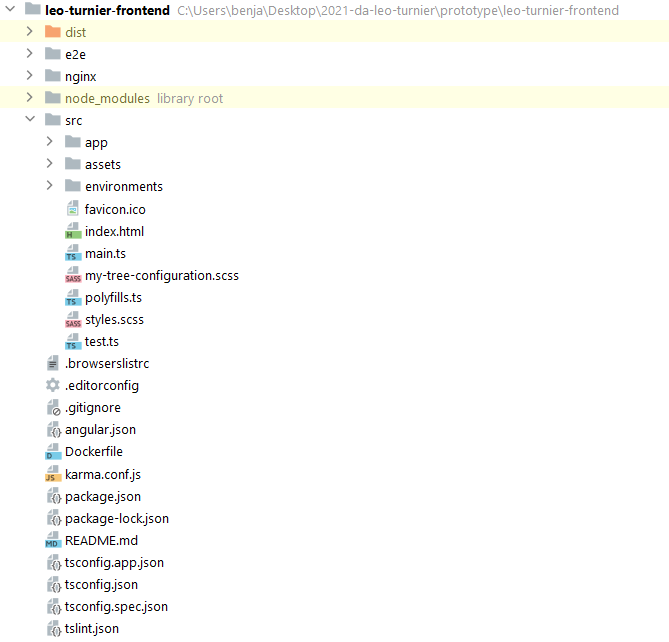
\includegraphics[scale=0.8]{pics/frontend/angular_file_structure.PNG}
    \caption{Angular Ordnerstruktur}
\end{figure}

Bei der Erstellung einer Angular Applikation wird schon fast die gesamte Ordnerstruktur festgelegt. Bis auf ein paar Ausnahmen wie der Nginx Ordner, oder die zwei in Gelb markierten Ordner,
welche nach dem dem Laden bzw. Builden generiert werden, hat sich hier nichts getan.
Wie an den meisten Filenamen schon zu erkennen ist befinden sich auf dieser Ebene so fast nur Files, die zur Konfiguration nötig sind. Das wichtigste File dabei ist "package.json".

\begin{figure}[H]
    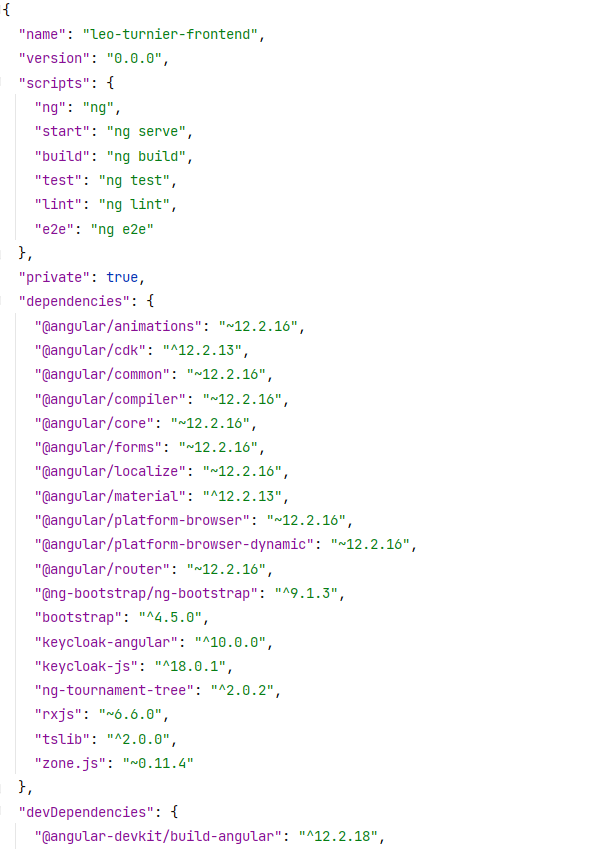
\includegraphics[scale=0.6]{pics/frontend/package_json.PNG}
    \caption{package.json}
\end{figure}

Hier werden alle Metadaten, Scripts und Dependencies der App aufgelistet.
Bei den Dependencies unterscheidet man zwischen Dependencies und DevDependencies.
\begin{itemize}
    \item Dependencies werden transitiv installiert: Wenn A B benötigt und B C benötigt, wird C installiert, sonst könnte B nicht funktionieren und A auch nicht.
    \item DevDependencies wird nicht transitiv installiert. Wir brauchen z.B. B nicht zu testen, um A zu testen, also können die Testabhängigkeiten von B weggelassen werden.
\end{itemize}

Um diese Dependencies auch nützen zu können muss bei jedem Angular Projekt "npm install" ausgeführt werden um diese zu Laden.
Danach werden sie dann im Ordner node\_modules gespeichert.
Dieser sollte, aber vor jeder Weitergabe gelöscht werden,oder wie zum Beispiel in Git im ".gitignore" inkludiert werden, da dieser mit Abstand am speicherintensivsten ist. 

\newpage
Auch wenn Angular eine große Anzahl an Ordnern und Files bietet geschieht wahrscheinlich 99\% der Arbeit eines Angular-Projekt im app Ordner.
Dieser enthält alle Components sowie Klassen die für die Applikation benötigt werden.

\begin{figure}[H]
    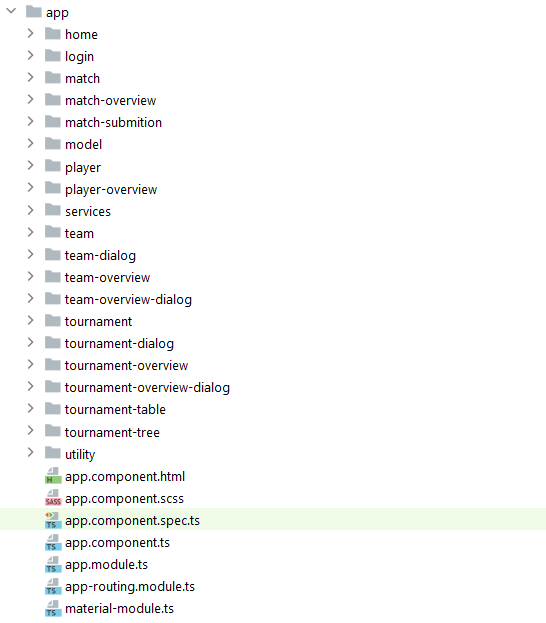
\includegraphics[scale=0.6]{pics/frontend/app_folder.PNG}
    \caption{App Ordner}
\end{figure}

Um ein bisschen Ordnung ins Chaos zu bringen kann man diese Files bzw Ordner in drei Kategorien unterteilen:
\begin{itemize}
    \item App Components: Alle Files die mit app anfangen
    \item Hilfklassen: model, services, utility, material-module.ts
    \item Components: Alle restlichen Ordner.
\end{itemize}

\subsection{App Components}
\subsubsection{Modules und Routing}

Modules und Routing sind der Kern einer Angular App. Hier laufen alle Components zusammen und 
Libraries werden über Imports eingebunden. Im Routing findet unter routes ein Array mit allen paths, sowie deren Components. Mit @NgModule wird das App-Modul erstellt.
Dort findet man dann auch alle Abhängigkeiten und Komponenten, die dieses Modul enthält. Um einen guten Überblick über alle Modules zu haben, wurden für die große Anzahl an AngularMaterial Modules ein eigens Module erstellt.
Beim Laden dieses Moduls wird der AppComponent gestartet. 
\cite{implementation-angular-1}

\begin{figure}[H]
    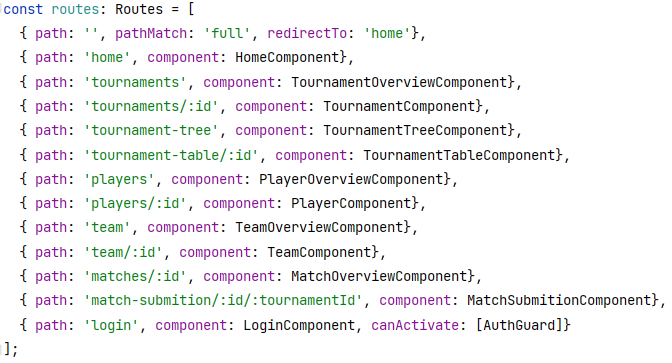
\includegraphics[scale=0.5]{pics/frontend/routes.PNG}
    \caption{routes in app-routing.module.ts}
\end{figure}

\begin{figure}[H]
    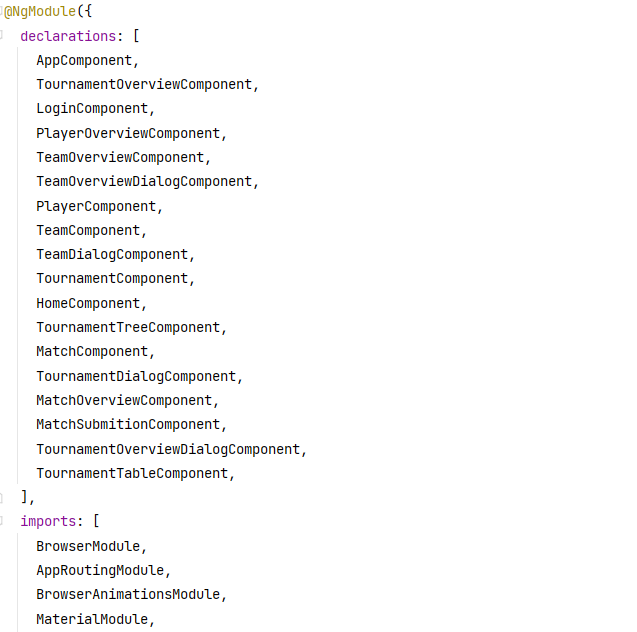
\includegraphics[scale=0.5]{pics/frontend/app_module.PNG}
    \caption{@NgModule in app.module.ts}
\end{figure}

\subsubsection{App-Component}

Die App Component ist der "Vater" jeder Angular App. Sie enthält alle anderen Child-Components und ist jederzeit sichtbar.
Daher eigent Sie sich perfekt für eine Tool- und Navbar. 
Wie alle Component besteht Sie aus 4 Files:
\begin{itemize}
    \item TypeScript (.ts): Ist der Code-Behind und enthält die gesamte Business Logik der Component. 
    \item HTML
    \item SCSS: Durch SCSS wird die Schreibweise von CSS vereinfacht und Variablen fest definiert.
    \item spec.ts: Die spec-Dateien sind Unit-Tests für den Sourcecode. Die Konvention für Angular-Anwendungen ist es, eine .spec.ts-Datei für jede .ts-Datei zu haben. \cite{implementation-angular-2}
\end{itemize}

\subsection{Hilfsklassen}
\subsubsection{Model}
Hier sind alle Klassen der App untergebracht. Bis auf ein paar Abweichung findet man hier das gleiche Datenmodel wie im Backend(7.1) wieder.
Da Angular mit Typescript verwendet wird, können für diese Klasse type checking verwendet werden (in vielen Fällen können stattdessen auch ein Interface verwendet werden)

\begin{figure}[H]
    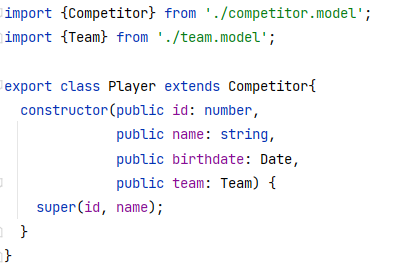
\includegraphics[scale=0.7]{pics/frontend/player_model.png}
    \caption{player.model.ts}
\end{figure}

\subsubsection{Services}
Components sollten Daten nicht direkt abrufen oder speichern. Sie sollten sich auf die Darstellung von Daten konzentrieren und den Datenzugriff an einen Service delegieren. In dem Ordner services befindet sich daher der gesamte Service, aufgeteilt in Aufgabenbereiche.
Jeder Service ist dabei gleich aufgebaut. Damit Angular den Service in eine Component injecten kann muss vorher ein Provider eingetragen werden. Ein Provider ist etwas, das einen Service erstellen oder bereitstellen kann.
Um sicherzustellen, dass der Service diesen anbieten kann, registrieren Sie ihn beim Injektor. Der Injektor ist das Objekt, das den Provider auswählt und dort injiziert, wo die Anwendung ihn benötigt.
Standardmäßig trägt Angular hierführ 'root' ein. Wenn ein Dienst auf Root-Ebene bereitgestellt wird, erstellt Angular eine einzelne, gemeinsam genutzte Instanz des Services und injiziert diese in jede Klasse, die danach fragt. \cite{implementation-angular-3}

Um Daten auf die Daten des Backends zugreifen zu können wird die Client-HTTP-API verwendet, welcher zugleich noch Features für Error-Handling und Typed Response Objects  bereitstellt. \cite{implementation-angular-4}

Da nicht jeder Nutzer von LeoTurnier Zugriff zu allen Daten haben darf, wird dazu noch ein Keycloak-Service verwendet der für jeden Request einen Authentication-Token zur Verfügung stellt.

\begin{figure}[H]
    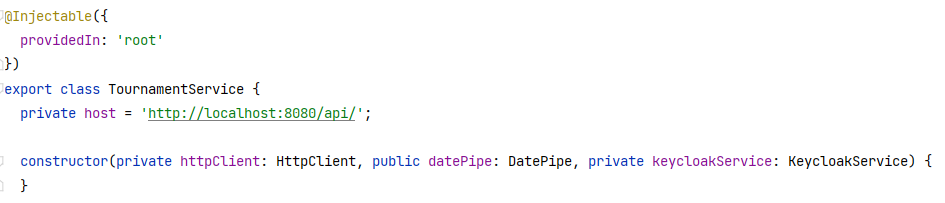
\includegraphics[scale=0.6]{pics/frontend/service.PNG}
    \caption{tournament.service.ts}
\end{figure}

\begin{figure}[H]
    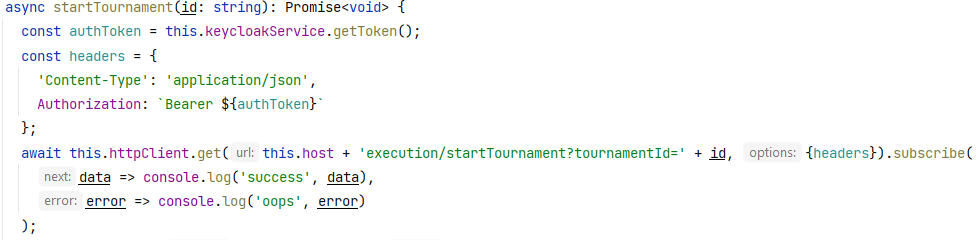
\includegraphics[scale=0.6]{pics/frontend/example_request.PNG}
    \caption{Beispiel Request: startTournament}
\end{figure}
